\subsubsection{Backpropagation 	algorithm and descent of the gradient in \acrshort{rnn}}
The calculation of the error in this type of architectures is the same as in the forward-pass networks, simply applying any cost function using as two arguments: the predicted value and the real value as explained in the section \ref{costfunction}. All calculated errors will be added up and saved in $C$. This error will be used to calculate the gradient of all the neurons. To do this it will be necessary to back-propagate the error. This error will be back-propagated in the same way as explained in the section \ref{backpropagation} for the non-recurrent layers.
\newline


For layers that apply some kind of loop, a new derivative must be added. To retropropagate the error, it is necessary to divide this error by proportional parts for each neuron. If, when adding the loop, a new connection is being added to itself, the error will have to be divided into two parts: one part for the previous layers and another for that same layer. Below you can see a diagram representing how the error is backpropagated. In summary, the error is back-propagated both in the network and in time, which is why this variant is called back-propagation through time.


\begin{figure}[H]
    \centering
    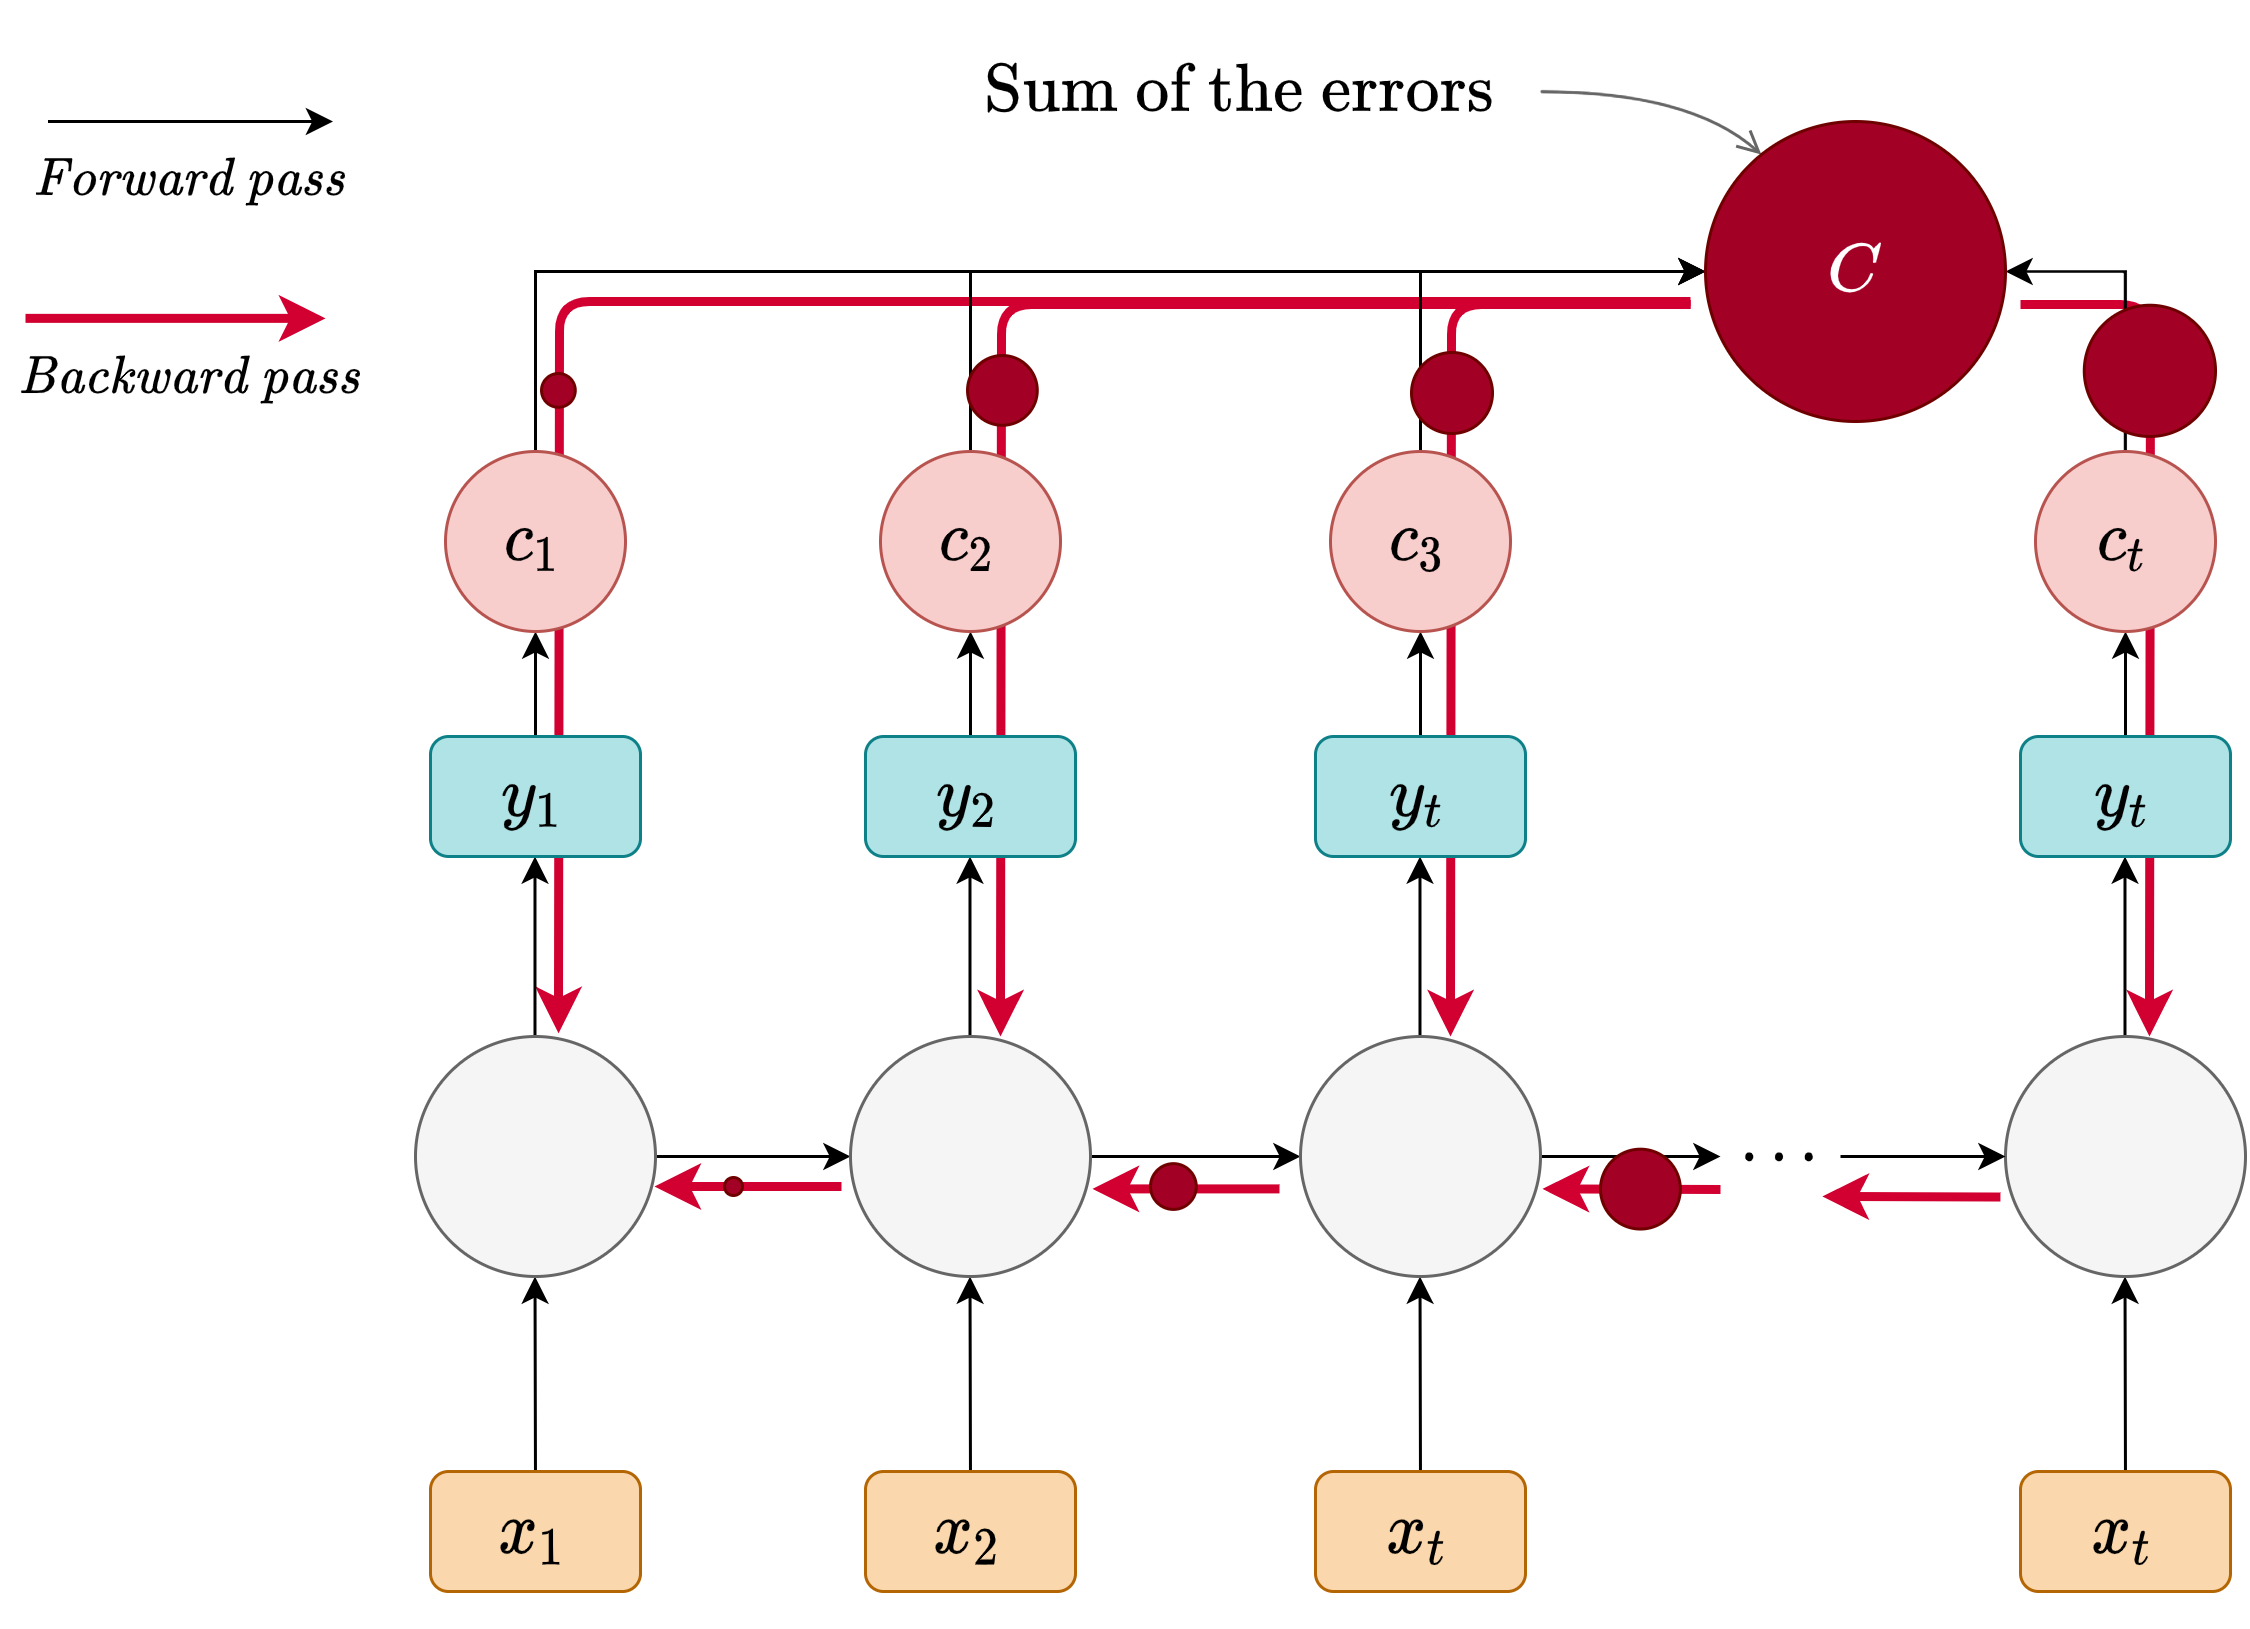
\includegraphics[width=14cm]{images/state-of-art/rnn/rnn-backward.png}
    \caption{Backpropagation over time in \acrshort{rnn}}
    \label{fig:Backpropagation_through_time}
\end{figure}

As can be seen, the error calculated $C$ from all the $c_i$, flow backwards in time. For the first part of the backpropagation calculation the same equations \ref{eqn:backpropagation_b} and \ref{eqn:backpropagation_w} can be used. In these equations the cost is calculated with respect to $w$ and with respect to $b$. The cost must be $C$ and not $c_i$. For the recurrent layers, a new derivative must be calculated: $\frac{\partial c}{\partial W_H}$. Applying the chain-rule as explained in section \ref{backpropagation}.

\begin{equation}
\begin{split}
     \frac{\partial C}{\partial W_h} &= \frac{\partial C}{\partial z^{L_i}} \cdot \frac{\partial z^{L_i}}{\partial W_h}
\end{split}
\label{eqn:backpropagation_h}
\end{equation}

And as in the gradient calculation made for $w$ and for $b$ in equation \ref{eqn:gradients}, the gradient of $W_H$ must be calculated in the same way:

\begin{equation}
    \nabla f_{w_h} = \begin{pmatrix} \frac{\partial C}{\partial w_h^{RL_1}}, & \frac{\partial C}{\partial w_h^{RL_2}}, & \cdots , &  \frac{\partial C}{\partial w_h^{RL_n}} \end{pmatrix}
\end{equation}

A detail to be emphasised is that $w_h$ is being used and not $W_H$, since the latter refers to the weight matrix of the recurrent layer. The gradient must be calculated independently for each neuron, as is the case with $w$ and $W$. This concept is explained in more detail in section \ref{workingwithmatrixes}. Once all $\nabla f_h$ have been calculated for each neuron, the weight matrix $w_{H}$ can be updated:

\begin{equation}
    \begin{split}
    H^* = H - \eta * \nabla f_{w_h}
    \end{split}
\end{equation}

It is important to first perform the backpropagation calculation and then perform the gradient calculation.
\newline
